\documentclass[11pt, a4paper, twoside]{article}   	% use "amsart" instead of "article" for AMSLaTeX format

\usepackage{geometry}                		% See geometry.pdf to learn the layout options. There are lots.
\usepackage{pdfpages}
\usepackage{caption}
\usepackage{minted}
\usepackage[german]{babel}			% this end the next are needed for german umlaute
\usepackage[utf8]{inputenc}
\usepackage{color}
\usepackage{graphicx}
\usepackage{titlesec}
\usepackage{fancyhdr}
\usepackage{lastpage}
\usepackage{hyperref}
% http://www.artofproblemsolving.com/wiki/index.php/LaTeX:Symbols#Operators
% =============================================
% Layout & Colors
% =============================================
\geometry{
   a4paper,
   total={210mm,297mm},
   left=20mm,
   right=20mm,
   top=20mm,
   bottom=30mm
 }	

\definecolor{myred}{rgb}{0.8,0,0}
\definecolor{mygreen}{rgb}{0,0.6,0}
\definecolor{mygray}{rgb}{0.5,0.5,0.5}
\definecolor{mymauve}{rgb}{0.58,0,0.82}

\setcounter{secnumdepth}{4}


% the default java directory structure and the main packages
\newcommand{\srcDir}{/src/main/java}
\newcommand{\srcTestDir}{/src/test/java}
\newcommand{\resourcesDir}{/src/main/resources}
\newcommand{\resourcesTestDir}{/src/test/resources}
\newcommand{\rmiAPISource}{../swe-campina-rmi-api\srcDir/at/fh/ooe/swe4/campina/rmi/api}
\newcommand{\rmiIMPLSource}{../swe-campina-rmi-impl\srcDir/at/fh/ooe/swe4/campina/rmi/impl}
\newcommand{\rmiRESSource}{../swe-campina-rmi-impl\resourcesDir}
\newcommand{\persAPISource}{../swe-campina-data-model-api\srcDir/at/fh/ooe/swe4/campina/persistence/api}
\newcommand{\persIMPLSource}{../swe-campina-data-model-impl\srcDir/at/fh/ooe/swe4/campina/persistence/impl}
\newcommand{\persRESSource}{../swe-campina-data-model-impl\resourcesDir}
\newcommand{\daoAPISource}{../swe-campina-dao-api\srcDir/at/fh/ooe/swe4/campina/dao}
\newcommand{\daoIMPLSource}{../swe-campina-dao-impl\srcDir/at/fh/ooe/swe4/campina/dao/impl}
\newcommand{\daoTESTSource}{../swe-campina-dao-impl\srcTestDir/at/fh/ooe/swe4/campina/test/dao}
\newcommand{\fxSource}{../swe-campina-fx\srcDir/at/fh/ooe/swe4/campina/fx}
% =============================================
% Code Settings
% =============================================
\newenvironment{code}{\captionsetup{type=listing}}{}
\newmintedfile[javaSourceFile]{java}{
	linenos=true, 
	frame=single, 
	breaklines=true, 
	tabsize=2,
	numbersep=5pt,
	xleftmargin=10pt,
	baselinestretch=1,
	fontsize=\footnotesize
}
\newmintinline[inlineJava]{java}{}
\newminted[javaSource]{java}{
	breaklines=true, 
	tabsize=2,
	autogobble=true,
	breakautoindent=false
}
\newmintedfile[xmlSourceFile]{xml}{
	linenos=true, 
	frame=single, 
	breaklines=true, 
	tabsize=2,
	numbersep=5pt,
	xleftmargin=10pt,
	baselinestretch=1,
	fontsize=\footnotesize
}
\newmintedfile[propertiesFile]{properties}{
	linenos=true, 
	frame=single, 
	breaklines=true, 
	tabsize=2,
	numbersep=5pt,
	xleftmargin=10pt,
	baselinestretch=1,
	fontsize=\footnotesize
}
\newmintedfile[sqlFile]{sql}{
	linenos=true, 
	frame=single, 
	breaklines=true, 
	tabsize=2,
	numbersep=5pt,
	xleftmargin=10pt,
	baselinestretch=1,
	fontsize=\footnotesize
}
% =============================================
% Page Style, Footers & Headers, Title
% =============================================
\title{Übung 3}
\author{Thomas Herzog}

\lhead{Übung 3}
\chead{}
\rhead{
\includegraphics[scale=0.10]{FHO_Logo_Students.jpg}}

\lfoot{S1310307011}
\cfoot{}
\rfoot{ \thepage / \pageref{LastPage} }
\renewcommand{\footrulewidth}{0.4pt}
% =============================================
% D O C U M E N T     C O N T E N T
% =============================================
\pagestyle{fancy}
\begin{document}
\setlength{\headheight}{15mm}
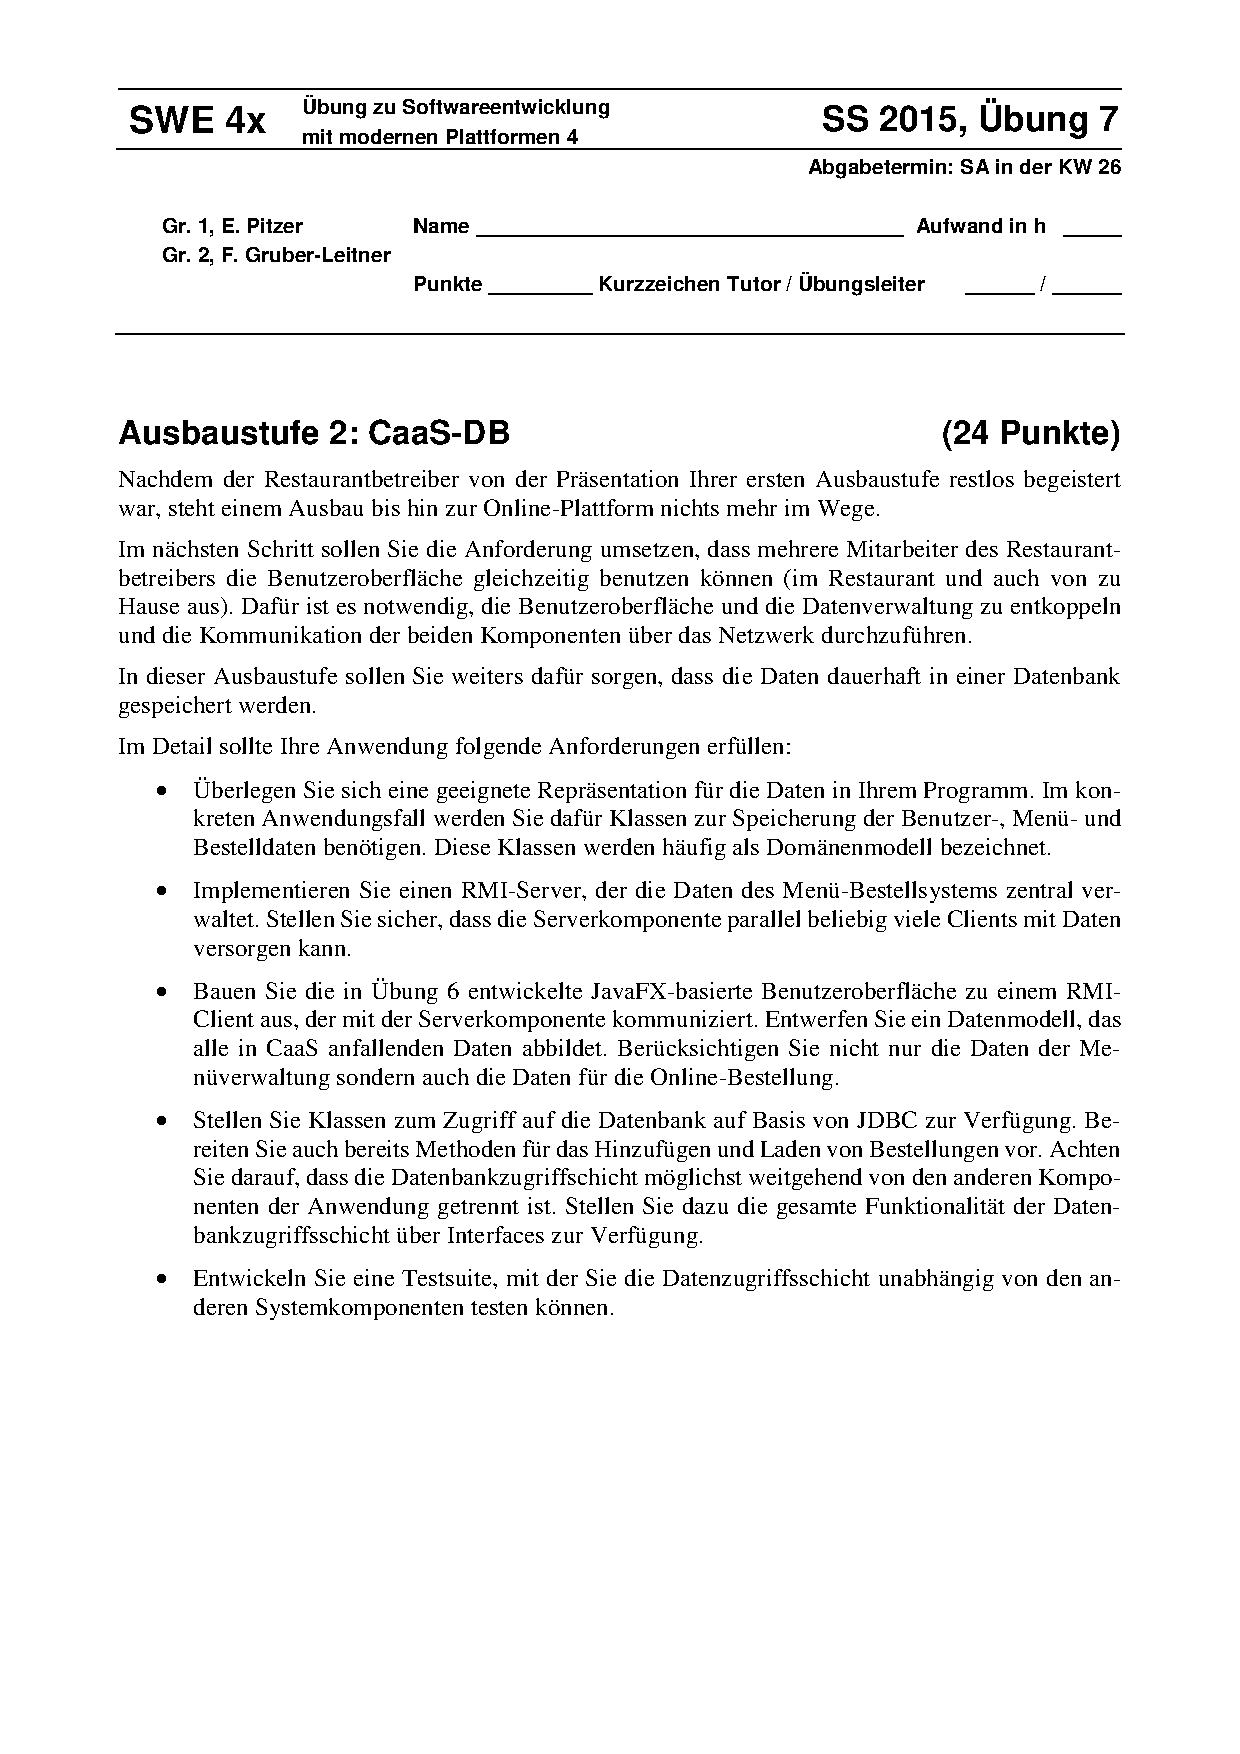
\includepdf[pages={1}]{Swe4xA07-BB.pdf}
{\color{myred}
	\section
		{Campina as a Service}
}

% =============================================
% Idea section
% =============================================
\subsection{Lösungsidee}
Folgend ist die Dokumentation der Aufgabenstellung Erweiterung CAAS angeführt.\\
Da hierbei mehrere Komponenten wie:
\begin{enumerate}
	\item RMI Server
	\item Domänen Modell
	\item DAOs für Domänen Modell
	\item UI mit JavaFx
\end{enumerate}
verwendet werden, soll die Gesamtapplikation in mehrere Projekte aufgeteilt werden.\\
Diese Projekte sollen wie folgt definiert werden:
\begin{enumerate}
	\item \emph{swe-campina-data-model-api}:\\
	Die API für das Domänen Modell und die Schnittstellen für den Datenzugriff. Es enthält keinen Datenbank spezifischen Source.
	\item \emph{swe-campina-data-model-impl}:\\
	Die Implementierung der API spezifiziert in \emph{swe-campina-data-model-api}. Stellt eine MySql spezifische Implementierung dar.
	\item \emph{swe-campina-dao-api}:\\
	Die API der DAOs für das Domänen Modell. Sind bereits hier Remote Schnittstellen.
	\item \emph{swe-campina-dao-impl}:\\
	Die Implementierung der API spezifiziert in \emph{swe-campina-dao-api}. Stellt eine MySql spezifische Implementierung dar.
	\item \emph{swe-campina-rmi-api}:\\
	Die API des RMI Servers, der die DAOs hostet.
	\item \emph{swe-campina-rmi-impl}:\\
	Die Implementierung der API spezifiziert in \emph{swe-campina-rmi-api}. Es hat Abhängigkeiten auf \emph{swe-campina-dao-api} und \emph{swe-campina-dao-impl}, da es diese Beans hostet.
	\item \emph{swe-campina-fx}:\\
	Die UI für CAAS in JavaFX. Hier sollen nur die Nötigen Änderungen vorgenommen werden um die Persistenz der Daten zu gewährleisten. 
\end{enumerate}
Folgend ein paar Informationen bezüglich dem Setup.
\subsubsection{RMI Server}
Im Projekt \emph{swe-campina-rmi-impl} gibt es eine Klasse names \emph{MainServer.java}. Diese startet den RMI Server und registriert die DAOFactory in der Registry. Diese Factory wird von den Clients genutzt um die DAOs zu produzieren, wobei pro Instanz maximal 10 Clients gebunden werden. Es nutzen jedoch alle dieselbe \inlineJava{ConnectionManager} Instanz.
\subsubsection{DAOs}
Im Projekt \emph{swe-campina-data-model-impl\resourcesDir} befindet sich das DDL \emph{create-campina-schema.sql}, die ausgeführt werden muss bevor das erste Mal eine der Applikationen gestartet wird. Des Weiteren ist dort eine Konfigurationsdatei namens \emph{db-config-properties} enthalten, welche die Konfigurationsparameter für den Verbindungsaufbau enthält, die im \inlineJava{ConnectionManager} genutzt werden. Diese Parameter werden über eine Enumeration \inlineJava{DbConfigParam} abgebildet, die auch die Properties Datei lädt. Diese muss auf Korrektheit geprüft werden bevor die Applikationen gestartet werden, um eine Datenbankverbindung gewährleisten zu können.\\
\subsubsection{UI}
Im Projekt \emph{swe-campina-fx} gibt es eine Klasse namens \emph{MainUI.java} welche die UI startet. Es werden Testdaten angelegt, sofern der Benutzer mit der Email \emph{thomas.herzog@students.fh-hagenberg.at} order mit dem Benutzernamen \emph{cchet} noch nicht auf der Datenbank existiert. Es werden hierbei auch die Orders für diesen Benutzer angelegt.
\subsubsection{JUnit Tests}
Für die DAOs wurde eine abstrakte Basisklasse eingeführt, welche eine Methode zur verfügung stellt welche die Datenbank neu erstellen kann. Sie nutzt dieselben Verbindungsdaten wie der Rest der Applikationen, daher ist anzumerken, das die Datenbank neu angelegt wird und daher alle Daten verloren gehen, was aber bei diesem Prototypen keine Rolle spielt, da Testdaten angelegt werden. 


% =============================================
% Source "swe-campina-data-model-api"
% =============================================
\newpage
\subsection{Source swe-campina-data-model-api}
Folgend ist der DSource des Projekts \emph{swe-campina-data-model-api} angeführt, welches die Spezifikation des Datenmodells darstellt, wobei hierbei keine Datenbank spezifischen Anteile enthalten sind.\\
Für das Mapping der Domänenmodelle gegen die Datenbanl wurden die JEE Annotations \inlineJava{@Table(), @Column} verwendet, da diese sich hierfür gut geeignet haben.
Es wird hierbei lediglich auf die Neuerungen eingegangen und der bestehende Source nicht nochmals dokumentiert.
\subsubsection{AbstractEntity.java}
Diese Klasse stellt die Wurzelklasse alle Entitäten dar. Sie enthält bereits eine \inlineJava{int hash(), boolean equals(Object other)} Implementierung.
\begin{code}
	\caption{AbstractEntity.java}
	\javaSourceFile{\persAPISource/AbstractEntity.java}
\end{code}

\subsubsection{ConnectionManager.java}
Dieses Interface spezifiziert den Verbindungsmanager der die Verbindungen verwaltet.
\begin{code}
	\caption{ConnectionManager.java}
	\javaSourceFile{\persAPISource/ConnectionManager.java}
\end{code}
\newpage

\subsubsection{EntityManager.java}
Dieses Interface spezifiziert den EntityManager, wobei jeweils eine Instanz für einen Typ eines Domänenmodells zuständig ist. Diese Spezifikation solles erleichtern mit den Entitäten und JDBC umzugehen.
\begin{code}
	\caption{EntityManager.java}
	\javaSourceFile{\persAPISource/EntityManager.java}
\end{code}
\newpage

\subsubsection{User.java}
Diese Klasse stellt den Benutzer auf der Datenbank da.
\begin{code}
	\caption{User.java}
	\javaSourceFile{\persAPISource/entity/User.java}
\end{code}
\newpage

\subsubsection{Menu.java}
Diese Klasse stellt die Menukarte auf der Datenbank da.
\begin{code}
	\caption{User.java}
	\javaSourceFile{\persAPISource/entity/Menu.java}
\end{code}
\newpage

\subsubsection{MenuEntry.java}
Diese Klasse stellt den Menu Eintrag auf der Datenbank da.
\begin{code}
	\caption{MenuEntry.java}
	\javaSourceFile{\persAPISource/entity/MenuEntry.java}
\end{code}
\newpage

\subsubsection{Order.java}
Diese Klasse stellt die Bestellung auf der Datenbank da.
\begin{code}
	\caption{Order.java}
	\javaSourceFile{\persAPISource/entity/Order.java}
\end{code}
\newpage


% =============================================
% Source "swe-campina-data-model-impl"
% =============================================
\subsection{Source swe-campina-data-model-impl}
Folgend ist die Implementierung der Spezifikation \emph{swe-campina-data-model-api} angeführt. Sie wurde auf eine MySql Datenbank ausgelegt.

\subsubsection{ConnectionManagerImpl.java}
Diese Klasse ist die Implementierung der Spezifikation \inlineJava{ConnectionManager} dar. Sie verwaltet die Verbindungen zu einer Datenbank.
\begin{code}
	\caption{ConnectionManagerImpl.java}
	\javaSourceFile{\persIMPLSource/ConnectionManagerImpl.java}
\end{code}
\newpage

\subsubsection{DbConfigParam.java}
Diese Enumeration spezifiziert die Parameter für die Konfigurationsdatei \emph{db-config.properties} und lädt diese auch.
\begin{code}
	\caption{DbConfigParam.java}
	\javaSourceFile{\persIMPLSource/DbConfigParam.java}
\end{code}
\newpage

\subsubsection{EntityManagerImpl.java}
Diese Klasse stellt die Implementierung der SPezifikation \inlineJava{EntityManager} dar. Sie soll den Übergang von Domänen Modell auf die Datenbank erleichtern, wobei sich hier sehr an JPA + Hibernate orientiert wurde.
\begin{code}
	\caption{EntityManagerImpl.java}
	\javaSourceFile{\persIMPLSource/EntityManagerImpl.java}
\end{code}
\newpage

\subsubsection{create-campina-schema.sql}
Diese Datei enthält die DDL Befehle zum Anlegen des Campina Schemas.
\begin{code}
	\caption{create-campina-schema.sql}
	\sqlFile{\persRESSource/create-campina-schema.sql}
\end{code}

\subsubsection{db-config.properties}
Diese Datei enthält die Konfiguration für JDBC.
\begin{code}
	\caption{db-config.properties}
	\sqlFile{\persRESSource/db-config.properties}
\end{code}
\newpage

% =============================================
% Source "swe-campina-dao-api"
% =============================================
\subsection{Source swe-campina-dao-api}
Folgend ist der Source des Projekts \emph{swe-campina-dao-api} angeführt, welcher die Sources für den Datenbankzugriff des Domänen Modells enthält. 

\subsubsection{AbstractRemoteDao.java}
Diese Klasse stellt die Wurzelklasse dar, von der alle Remote DAOs erben.
\begin{code}
	\caption{AbstractRemoteDao.java}
	\javaSourceFile{\daoAPISource/api/AbstractRemoteDao.java}
\end{code}
\newpage

\subsubsection{RemoteDao.java}
Dieses Interface spezifiziert die Mindestanfordernungen an ein DAO. Es enthält alle Operationen, die für einen Entity anwendbar sein müssen.
\begin{code}
	\caption{RemoteDao.java}
	\javaSourceFile{\daoAPISource/api/RemoteDao.java}
\end{code}

\subsubsection{UserDao.java}
Diese Interface spezifiziert die DAO Methoden für den Entitätentyp User.
\begin{code}
	\caption{UserDao.java}
	\javaSourceFile{\daoAPISource/api/UserDao.java}
\end{code}

\subsubsection{MenuDao.java}
Diese Interface spezifiziert die DAO Methoden für den Entitätentyp Menu.
\begin{code}
	\caption{MenuDao.java}
	\javaSourceFile{\daoAPISource/api/MenuDao.java}
\end{code}
\newpage

\subsubsection{MenuEntryDao.java}
Diese Interface spezifiziert die DAO Methoden für den Entitätentyp MenuEntry.
\begin{code}
	\caption{MenuEntryDao.java}
	\javaSourceFile{\daoAPISource/api/MenuEntryDao.java}
\end{code}

\subsubsection{OrderDao.java}
Diese Interface spezifiziert die DAO Methoden für den Entitätentyp Order.
\begin{code}
	\caption{OrderDao.java}
	\javaSourceFile{\daoAPISource/api/OrderDao.java}
\end{code}
\newpage

\subsubsection{EmailAlreadyUsedException.java}
Diese Exception zeigt dem Client an, dass eine Email bereits verwendet wurde.
\begin{code}
	\caption{EmailAlreadyUsedException.java}
	\javaSourceFile{\daoAPISource/exception/EmailAlreadyUsedException.java}
\end{code}
\newpage

\subsubsection{UsernameAlreadyUsedException.java}
Diese Exception zeigt dem Client an, dass ein Benutzername bereits verwendet wurde.
\begin{code}
	\caption{UsernameAlreadyUsedException.java}
	\javaSourceFile{\daoAPISource/exception/UsernameAlreadyUsedException.java}
\end{code}
\newpage

% =============================================
% Source "swe-campina-dao-impl"
% =============================================
\subsection{Source swe-campina-dao-impl}
Folgend ist der Source des Projekts \emph{swe-campina-dao-impl} angeführt, welches die Implementierung der Spezifikation \emph{swe-campina-dao-api} darstellt. 

\subsubsection{UserDaoImpl.java}
Diese Klasse stellt die Implementierung der Spezifikation \inlineJava{UserDao} dar.
\begin{code}
	\caption{UserDaoImpl.java}
	\javaSourceFile{\daoIMPLSource/UserDaoImpl.java}
\end{code}
\newpage

\subsubsection{MenuDaoImpl.java}
Diese Klasse stellt die Implementierung der Spezifikation \inlineJava{MenuDao} dar.
\begin{code}
	\caption{MenuDaoImpl.java}
	\javaSourceFile{\daoIMPLSource/MenuDaoImpl.java}
\end{code}
\newpage

\subsubsection{MenuEntryDaoImpl.java}
Diese Klasse stellt die Implementierung der Spezifikation \inlineJava{MenuEntryDao} dar.
\begin{code}
	\caption{MenuEntryDaoImpl.java}
	\javaSourceFile{\daoIMPLSource/MenuEntryDaoImpl.java}
\end{code}
\newpage

\subsubsection{OrderDaoImpl.java}
Diese Klasse stellt die Implementierung der Spezifikation \inlineJava{OrderDao} dar.
\begin{code}
	\caption{OrderDaoImpl.java}
	\javaSourceFile{\daoIMPLSource/OrderDaoImpl.java}
\end{code}
\newpage

\subsubsection{AbstractDaoTest.java}
Diese abstrakte Klasse stellt die Wurzelklasse aller DAO Test Implementierungen dar. Sie stellt Methoden für das Anlegen einer Datenbank zu Verfügung, was in den folgenden Tests vor und nachdem Test passiert.
\begin{code}
	\caption{AbstractDaoTest.java}
	\javaSourceFile{\daoTESTSource/api/AbstractDaoTest.java}
\end{code}
\newpage

\subsubsection{RemoteDetailMatcher.java}
Diese Klasse ist eine Hilfsklasse, die über eine JUnit Rule auf Excptions reagiert, damit Causes getestet werden können, da die DAOs immer \inlineJava{RemoteException} werfen.
\begin{code}
	\caption{RemoteDetailMatcher.java}
	\javaSourceFile{\daoTESTSource/api/RemoteDetailMatcher.java}
\end{code}
\newpage

\subsubsection{RemoteExceptionLogger.java}
Diese Klasse ist eine Hilfsklasse, die über eine JUnit Rule auf Excptions reagiert, damit Causes geloggt werden können, da die DAOs immer \inlineJava{RemoteException} werfen, wobei dessen Member \inlineJava{remoteExc.detail} die eigentliche Cause enthält.
\begin{code}
	\caption{RemoteExceptionLogger.java}
	\javaSourceFile{\daoTESTSource/api/RemoteExceptionLogger.java}
\end{code}
\newpage

\subsubsection{UserDaoTest.java}
Diese Testklasse testet das DAO \inlineJava{UserDao}
\begin{code}
	\caption{UserDaoTest.java}
	\javaSourceFile{\daoTESTSource/impl/UserDaoTest.java}
\end{code}
\newpage

\subsubsection{MenuDaoTest.java}
Diese Testklasse testet das DAO \inlineJava{MenuDao}
\begin{code}
	\caption{MenuDaoTest.java}
	\javaSourceFile{\daoTESTSource/impl/MenuDaoTest.java}
\end{code}
\newpage

\subsubsection{MenuEntryDaoTest.java}
Diese Testklasse testet das DAO \inlineJava{MenuEntryDao}
\begin{code}
	\caption{MenuEntryDaoTest.java}
	\javaSourceFile{\daoTESTSource/impl/MenuEntryDaoTest.java}
\end{code}
\newpage

\subsubsection{OrderDaoTest.java}
Diese Testklasse testet das DAO \inlineJava{OrderDaoTest}
\begin{code}
	\caption{OrderDaoTest.java}
	\javaSourceFile{\daoTESTSource/impl/OrderDaoTest.java}
\end{code}
\newpage

% =============================================
% Source "swe-campina-rmi-api"
% =============================================
\subsection{Source swe-campina-rmi-api}
Folgend ist der Source des Projekts \emph{swe-campina-rmi-api} angeführt, welches die Spezifikation für den RMI Server darstellt.

\subsubsection{RmiServer.java}
Dieses Interface spezifiziert den RMI Server.
\begin{code}
	\caption{RmiServer.java}
	\javaSourceFile{\rmiAPISource/rmi/RmiServer.java}
\end{code}

\subsubsection{RmiDaoFactory.java}
Dieses Interface spezifiziert die RMI DAO Factory.
\begin{code}
	\caption{RmiDaoFactory.java}
	\javaSourceFile{\rmiAPISource/factory/RmiDaoFactory.java}
\end{code}
\newpage


% =============================================
% Source "swe-campina-rmi-impl"
% =============================================
\subsection{Source swe-campina-rmi-impl}
Folgend ist der Source des Projekts \emph{swe-campina-rmi-impl} angeführt, welches die Implementierung der Spezifikation \emph{swe-campina-rmi-impl}.

\subsubsection{RmiServerImpl.java}
Diese Klasse stellt die Implementierung der Spezifikation \emph{RmiServer} dar.
\begin{code}
	\caption{RmiServerImpl.java}
	\javaSourceFile{\rmiIMPLSource/RmiServerImpl.java}
\end{code}
\newpage

\subsubsection{RmiDaoFactoryImpl.java}
Diese Klasse stellt die Implementierung der Spezifikation \emph{RmiDaoFactory} dar.
\begin{code}
	\caption{RmiDaoFactoryImpl.java}
	\javaSourceFile{\rmiIMPLSource/RmiDaoFactoryImpl.java}
\end{code}
\newpage

\subsubsection{MainServer.java}
Diese Klasse stellt die Main Klasse für den RMI Server dar.
\begin{code}
	\caption{MainServer.java}
	\javaSourceFile{\rmiIMPLSource/MainServer.java}
\end{code}

\subsubsection{log4j.properties}
Die Konfigurationsdatei für Log4j für die RMI Server hosting JVM.
\begin{code}
	\caption{log4j.properties}
	\propertiesFile{\rmiRESSource/log4j.properties}
\end{code}
\newpage

% =============================================
% Source "swe-campina-fx"
% =============================================
\subsection{Source swe-campina-fx}
Folgend ist der Source des Projekts \emph{swe-campina-fx} angeführt, wobei hier nur die Klassen, in dennen Änderungen vorgenommen wurden angeführt sind.\\
Die Domänen Modelle, die bereits vorhanden waren, wurden in das Projekt \emph{swe-campina-data-model-api} verschoben. Die Simulation der Datenbank wurde entfernt.

\subsubsection{UserEventControl.java}
Diese Klasse für die Events bezüglich der Entität \inlineJava{User}.
\begin{code}
	\caption{UserEventControl.java}
	\javaSourceFile{\fxSource/view/admin/user/control/UserEventControl.java}
\end{code}
\newpage

\subsubsection{MenuEventControl.java}
Diese Klasse für die Events bezüglich der Entität \inlineJava{Menu}.
\begin{code}
	\caption{MenuEventControl.java}
	\javaSourceFile{\fxSource/view/admin/menu/control/MenuEventControl.java}
\end{code}
\newpage

\subsubsection{MenuEntryEventControl.java}
Diese Klasse für die Events bezüglich der Entität \inlineJava{MenuEntry}.
\begin{code}
	\caption{MenuEntryEventControl.java}
	\javaSourceFile{\fxSource/view/admin/menu/control/MenuEntryEventControl.java}
\end{code}
\newpage

\subsubsection{MainFX.java}
Diese Klasse stellt die Main Klasse für die JavaFX Applikation dar.
\begin{code}
	\caption{MainFX.java}
	\javaSourceFile{\fxSource/main/MainFX.java}
\end{code}
\newpage


% =============================================
% Test "swe-campina-dao-impl"
% =============================================
\subsection{Test swe-campina-dao-impl}
Folgend sind die Tests für das Projekt \emph{swe-campina.dao-impl} angeführt, wobei hier lediglich die JUnit Tests aus Eclipse angeführt sind.\\
Die DAOs können ohne weitere Infrastruktur getestet werden, und die Test haben zwar Abhängigkeiten auf RMI spezifische API jedoch ist kein registrieren der DAOs über RMI erforderlich.
  
\begin{figure}[h]
	\centering
	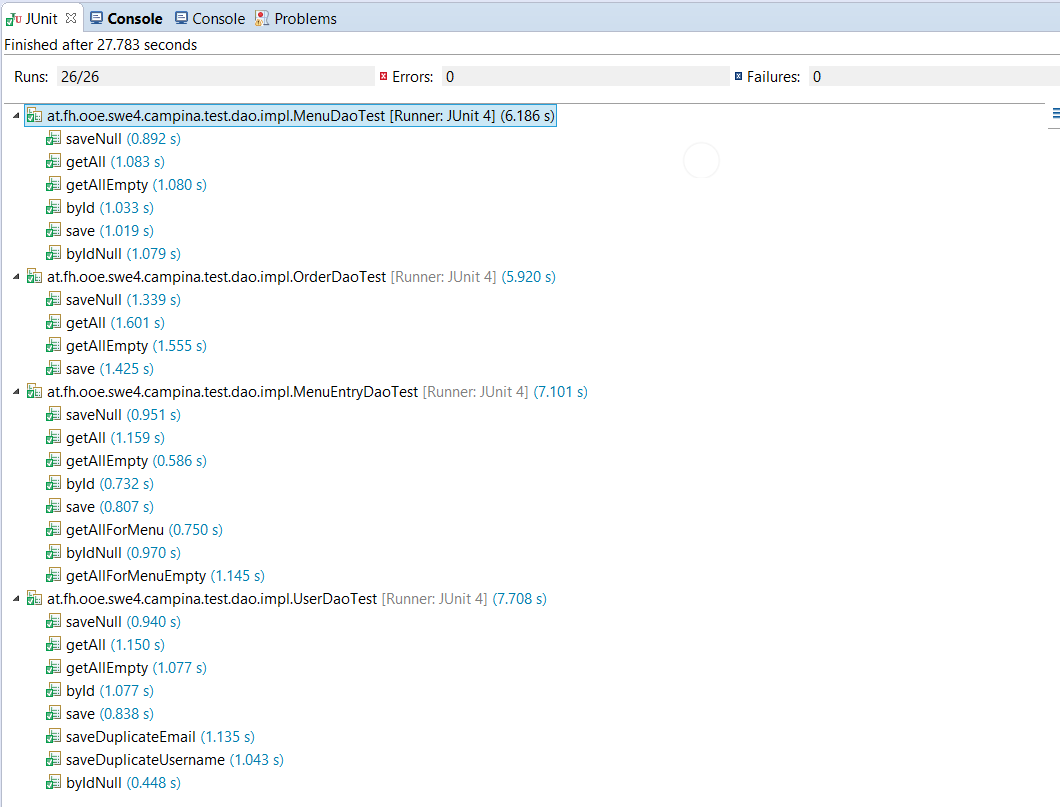
\includegraphics[scale=0.7]{images/dao-test.PNG}
	\caption
	{Die JUnit Test aus Eclipse}
\end{figure}
\newpage 
\end{document}  